\documentclass[xetex,mathserif,serif]{beamer}
\usepackage{polyglossia}
\setdefaultlanguage[babelshorthands=true]{russian}
\usepackage{minted}

\useoutertheme{infolines}

\setmainfont{FreeSans}
\newfontfamily{\russianfonttt}{FreeSans}

\definecolor{links}{HTML}{2A1B81}
\hypersetup{colorlinks,linkcolor=,urlcolor=links}

\title{Учебные практики на кафедре СП}
\subtitle{Требования, рекомендации}
\author[Юрий Литвинов]{Юрий Литвинов \newline \textcolor{gray}{\small\texttt{y.litvinov@spbu.ru}}}
\date{15.09.2021}

\begin{document}
    
    \frame{\titlepage}

    \begin{frame}
        \frametitle{Что такое учебная практика}
        \begin{itemize}
            \item Научно-исследовательская или программно-инженерная работа
            \begin{itemize}
                \item Решение более-менее научной или практически полезной задачи
                \item Отчёт (текст)
                \item Код
                \item Выступление на защите
            \end{itemize}
            \item По формату близка к научной статье и выступлению на конференции
            \item На два семестра, с промежуточной отчётностью зимой
            \item Тема должна быть интересна кафедре (``программирование для программистов'')
        \end{itemize}
    \end{frame}

    \begin{frame}
        \frametitle{Требования, осень}
        \begin{itemize}
            \item Отчёт на 10-15 страниц
            \begin{itemize}
                \item Введение, постановка задачи, обзор, начало реализации, план апробации/экспериментов
                \item Выполненные задачи, задачи на весну
                \item Будет выборочное рецензирование!
            \end{itemize}
            \item Доклад
            \begin{itemize}
                \item Порядка 3-5 минут
                \item Рассказать о задаче и текущих успехах
            \end{itemize}
            \item Отзывы научного руководителя и консультанта
            \item Ссылка на код, если он открыт
            \begin{itemize}
                \item Должен быть грамотно оформлен репозиторий
                \item Ссылка на репозиторий в заключении отчёта
            \end{itemize}
        \end{itemize}
    \end{frame}

    \begin{frame}
        \frametitle{Требования, весна}
        \begin{itemize}
            \item Отчёт на 20-30 страниц
            \begin{itemize}
                \item Полное описание работы, включая осеннюю часть
                \item Можно переиспользовать текст осенних практик
                \item Тоже будет выборочное рецензирование
            \end{itemize}
            \item Доклад, на 7-9 минут
            \begin{itemize}
                \item Предзащита
                \item Защита
            \end{itemize}
            \item Снова отзывы, ссылку на код в заключение
        \end{itemize}
    \end{frame}

    \begin{frame}
        \frametitle{Кто такой научник, консультант и т.п.?}
        \begin{itemize}
            \item \textit{Консультант} --- ставит задачу, читает и рецензирует код, помогает с техническими проблемами
            \item \textit{Научный руководитель} --- преподаватель (обязательно), отвечает за адекватность задачи, следит за методологическими вопросами, следит за ходом работы, помогает с текстом и подготовкой к защите
            \item \textit{Руководитель практики} --- общая организация процесса, сбор и распределение тем, сбор отчётов и отзывов, организация защит, решение организационных проблем
            \item \textit{Комиссия} --- преподаватели кафедры, представитель индустрии
            \begin{itemize}
                \item Все защиты всегда с комиссией
                \item \emph{Защищаетесь в комиссии той кафедры, с которой научник}
            \end{itemize}
        \end{itemize}
    \end{frame}

    \begin{frame}
        \frametitle{Откуда брать тему и научного руководителя}
        \begin{itemize}
            \item Глобальная таблица с темами: \url{https://bit.ly/themes-2021-2022}
            \begin{itemize}
                \item Обратите внимание, там вкладки по кафедрам
                \item Ищите те, про которые написано, что они могут быть практиками третьего курса
                \item Если тема заинтересовала, но не подходит, можно пообщаться с консультантом
            \end{itemize}
            \item На стажировке, работе
            \item Результат выбора темы \textbf{до конца сентября} записать сюда: \url{https://bit.ly/practices-3rd-course}
            \begin{itemize}
                \item Там тоже вкладки по кафедрам
            \end{itemize}
        \end{itemize}
    \end{frame}

    \begin{frame}
        \frametitle{Полезные ресурсы}
        \begin{itemize}
            \item Рассылка кафедры: \url{http://bit.ly/sysprog-talks}
            \item Рассылка курса СП: \url{https://groups.google.com/g/spbsu-se-bachelors-2019-2023}
            \item Команда Teams СП: \textbf{xao59z5}
            \item Команда Teams матобеса: \textbf{5xdod4t}
            \begin{itemize}
                \item Подписаться и включить уведомления обязательно
            \end{itemize}
            \item Сайт кафедры --- \url{https://se.math.spbu.ru/}
            \begin{itemize}
                \item Раздел ``Студентам'' --- архив работ
            \end{itemize}
            \item Шаблон отчёта: \url{https://github.com/spbu-se/matmex-diploma-template}
            \item Шаблон презентации: \url{https://github.com/spbu-se/report_presentation_template}
            \item Онлайн-редакторы TeX --- \url{https://papeeria.com/}, \url{https://www.overleaf.com/}
        \end{itemize}
    \end{frame}

    \begin{frame}
        \frametitle{Примерный план, осенний семестр}
        \begin{itemize}
            \item Сентябрь --- определиться с научным руководителем и темой
            \item Работа над практикой
            \begin{itemize}
                \item Быстрый мини-обзор
                \item Введение, постановка задачи, научиться убеждать окружающих в актуальности темы
                \item Обзор
                \item Проектирование
                \item Написание текста
            \end{itemize}
            \item Середина декабря --- сдача текста на выборочное рецензирование
            \item Конец декабря --- защиты
        \end{itemize}
    \end{frame}

    \begin{frame}
        \frametitle{Примерный план, весенний семестр}
        \begin{itemize}
            \item Февраль--май --- работа над практикой
            \begin{itemize}
                \item Реализация
                \item Апробация/эксперименты
                \item Написание текста
            \end{itemize}
            \item Начало мая --- предзащиты
            \item Начало--середина мая --- выборочное рецензирование
            \item Конец мая --- защиты
            \item Минимум раз в неделю отчитываться научному руководителю о ходе работы
            \item Весенние отчёты публикуются на сайте кафедры
        \end{itemize}
    \end{frame}

    \begin{frame}
        \frametitle{Отчёт, структура}
        \begin{itemize}
            \item Титульный лист
            \item Оглавление
            \item Введение в предметную область, постановка задачи
            \item Обзор литературы и существующих решений
            \item Описание предлагаемого решения (архитектура, план реализации, что успели сделать)
            \item Заключение
            \item Список литературы
        \end{itemize}
    \end{frame}

    \begin{frame}
        \frametitle{Введение}
        \begin{columns}
            \begin{column}{0.6\textwidth}
                \begin{itemize}
                    \item Известная информация, ``Background''
                    \item Неизвестная информация, ``Gap''
                    \begin{itemize}
                        \item Актуальность темы
                        \item Практическая значимость
                        \item Кому конкретно это надо
                    \end{itemize}
                    \item Кратко про ваш подход к решению задачи, почему он приведёт к успеху (``Гипотеза'' и ``Подход'')
                \end{itemize}
            \end{column}
            \begin{column}{0.4\textwidth}
                \begin{center}
                    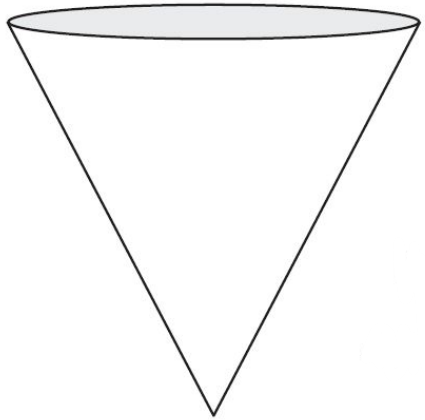
\includegraphics[width=\textwidth]{introductionCone.png}
                \end{center}
            \end{column}
        \end{columns}
    \end{frame}

    \begin{frame}
        \frametitle{Постановка задачи}
        \begin{itemize}
            \item Цель работы
            \begin{itemize}
                \item Одним предложением --- что конкретно надо сделать
            \end{itemize}
            \item Задачи
            \begin{itemize}
                \item Отчуждаемые
                \item Специфичные
                \item Решение которых приведёт к цели
                \item Выполнить обзор, спроектировать, реализовать, выполнить апробацию/эксперименты
                \item Отдельно на осеннюю и весеннюю часть
            \end{itemize}
        \end{itemize}
    \end{frame}

    \begin{frame}
        \frametitle{Обзор}
        \begin{itemize}
            \item Обзор существующих решений
            \begin{itemize}
                \item Цель обзора, критерии отбора материалов
                \item Критерии сравнения
                \item Таблица с результатами
                \item Выводы
            \end{itemize}
            \item Обзор используемых чужих результатов
            \begin{itemize}
                \item  Всё, написанное и придуманное не вами --- в обзор
            \end{itemize}
            \item Должен соотноситься с темой работы
        \end{itemize}
    \end{frame}

    \begin{frame}
        \frametitle{Описание решения}
        \begin{itemize}
            \item Весной будет несколько разделов, сейчас достаточно одного
            \begin{itemize}
                \item Желательно, чтобы разделы соответствовали списку задач
            \end{itemize}
            \item Аргументированное обоснование принятых решений и отказа от альтернатив
            \item Выбор инструментария
            \item Описание архитектуры, алгоритмов и т.п.
        \end{itemize}
    \end{frame}

    \begin{frame}
        \frametitle{Общие рекомендации}
        \begin{itemize}
            \item Никакого заимствования 
            \begin{itemize}
                \item Сдача чужой работы --- отчисление без права восстановления сразу
                \item Копипаст даже одного предложения без указания источника --- незачёт
                \item Правильно оформленный копипаст --- попросят убрать
            \end{itemize}
            \item Обязательно показать и текст, и презентацию научному руководителю
            \begin{itemize}
                \item Стоит порепетировать выступление
            \end{itemize}
            \item Из презентации должно быть предельно понятно, что и зачем вы делаете (актуальность, сложность работы) и при чём тут СП
            \begin{itemize}
                \item Будут яростно нападать
            \end{itemize}
            \item Озаботьтесь получением отзывов заранее
            \item Код --- CI, юнит-тесты, README, лицензия
        \end{itemize}
    \end{frame}

    \begin{frame}
        \frametitle{FAQ}
        \begin{small}
            \begin{itemize}
                \item Можно ли писать групповую практику?
                \begin{itemize}
                    \item Да, но отчёт и презентация у каждого свои
                \end{itemize}
                \item Засчитывают ли выступление на семинаре/конференции за защиту?
                \begin{itemize}
                    \item Нет
                \end{itemize}
                \item Можно ли менять тему и научника?
                \begin{itemize}
                    \item Да, но предупредить руководителя практики
                \end{itemize}
                \item Можно ли перезачесть работу, написанную в прошлом году?
                \begin{itemize}
                    \item Да, но тоже предупредить
                \end{itemize}
                \item Если научник/консультант/лаборатория/бомж с улицы ставит мне зачёт, как его получить в зачётку?
                \begin{itemize}
                    \item Никак, учебные практики принимаются комиссией в рамках процедуры независимой оценки качества образования
                \end{itemize}
                \item А ещё курсовая?
                \begin{itemize}
                    \item Нет, вместо курсовых теперь практики
                \end{itemize}
            \end{itemize}
        \end{small}
    \end{frame}

\end{document}